\documentclass[conference]{IEEEtran}
\hyphenation{op-tical net-works semi-conduc-tor IEEEtran}
\usepackage[bottom=2cm,top=3cm,left=3cm,right=2cm]{geometry}
\usepackage{url}
\makeatletter
\def\ps@pprintTitle{%
	\let\@oddhead\@empty
	\let\@evenhead\@empty
	\def\@oddfoot{\reset@font\hfil\thepage\hfil}
	\let\@evenfoot\@oddfoot
}
\makeatother

\usepackage{babelbib}

\usepackage[brazilian]{babel} % Traduz alguns termos para o português
\usepackage[utf8]{inputenc} % Reconhece acentuação
\usepackage{setspace}
\usepackage{graphicx}


\begin{document}

% paper title
\title{Teoria da Decisão\\ Métodos Escalares de Otimização Vetorial e Tomada de Decisão Assistida}


% author names and affiliations
% use a multiple column layout for up to three different
% affiliations
\author{\authorblockN{Rafael Carneiro de Castro}
\authorblockA{\\Engenharia de Sistemas - UFMG\\
Matrícula: 2013030210\\
Email: rafaelcarneiroget@hotmail.com}
\and
\authorblockN{Davi Pinheiro Viana}
\authorblockA{\\Engenharia de Sistemas - UFMG\\
	Matrícula: 2013029912\\
	Email: daviviana22@gmail.com}}

\maketitle

\begin{abstract}
Abordagem de forma conjunta de grande parte dos conceitos vistos na disciplina "ELE088 - Teoria da Decisão", através de um problema de escalonamento de tarefas.
\end{abstract}

\IEEEpeerreviewmaketitle



\section{Introdução}
O presente trabalho tem o objetivo de resolver um problema de otimização utilizando as técnicas escalares e de decisão assistida estudados em sala de aula, colocando em prática grande parte dos conceitos da matéria.

O problema a ser resolvido é o seguinte:
\textit{Uma empresa possui um conjunto de M máquinas que devem ser utilizadas para processar N tarefas indivisíveis. Cada máquina $i$ leva um tempo $t_{ij}$ para processar uma tarefa $j$ e pode processar uma única tarefa por vez. Todas as tarefas possuem uma mesma data ideal de entrega $d$, sendo que cada tarefa $j$ sofre uma penalidade $w_j$ proporcional a cada dia que ela é entregue adiantada ou atrasada em relação a $d$.}

\subsection{Formulação do Problema:}
A formulação do problema foi dividida em duas partes, como é discutido a seguir:

\subsubsection{Minimização do Tempo Total de Entrega}
Em primeiro momento é preciso construir uma função objetivo e suas eventuais restrições para minimização do tempo total de entrega de todas as tarefas. Considere $C_i$ como sendo o tempo necessário para se terminar as tarefas executadas pela máquina $i$. Assim:
\[C_i = \sum_{j=1}^{N}t_{ij}*x_{ij}\ \forall\ i \in\ (1,...,M) \]
O objetivo então se torna:
\[min\ C_{max} \]
\[C_{max} = max(C_i)\ \forall\ i \in\ (1,...,M) \]
sujeito a:
\[\sum_{i=1}^{M}x_{ij}=1\ \forall\ j \in\ (1,...,N) \]
\[\sum_{j=1}^{N}t_{ij}*x_{ij} <= C_{max}\ \forall\ i \in\ (1,...,M) \]
\[X_{ij} \in (0, 1) \]
Com estas restrições, garante-se que cada tarefa vai ser cumprida por uma única máquina. A matriz $x$ é composta por zeros e uns. Cada uma das suas linhas, então, vai representar uma tarefa, e cada coluna, uma máquina. O número 1 em uma linha representa qual máquina vai executar a tarefa daquela linha.

\subsubsection{Minimização da Soma Ponderada dos Atrasos e Adiantamentos}
Agora, uma função objetivo para tratar a minimização da soma ponderada dos atrasos e adiantamentos é formulada. O momento de término da tarefa $j$ será chamado de $e_j$. Então:
\[e_j = \sum_{i=1}^{M}t_{ik}\ \forall\ k \in\ \Omega_i \]
onde $\Omega_i$ é o conjunto das tarefas até a tarefa $i$. A função objetivo pode ser escrita como:
\[min\ \sum_{j=1}^{N}w_j|e_j-d| \]
sujeito a:
\[\sum_{i=1}^{M}x_{ij}=1\ \forall\ j \in\ (1,...,N) \]
\[X_{ij} \in (0, 1) \]
onde, como já discutido, $d$ é a data ideal de entrega das tarefas e $w_j$ a penalidade proporcional a cada dia que a tarefa é entregue adiantada ou atrasada em relação a $d$.

\subsection{Algoritmos de Solução:}
Nesta seção serão discutidos e exibidos os algoritmos para solução dos problemas mono e multi objetivo.
\subsubsection{Minimização do Tempo Total de Entrega}
O algoritmo de otimização utilizado aqui se baseia no \textit{Simulated Annealing}, método estudado em sala de aula de fácil implementação e convergência atrativa. Este método escapa de mínimos locais com a aceitação de alguns movimentos de piora na qualidade da solução. É inspirado no recozimento físico de sólidos, e possui um parâmetro conhecido como \textit{temperatura}, que ajusta a probabilidade de um movimento de piora ser aceito. Um algoritmo simplificado para o \textit{Simulated Annealing} pode ser visto na Figura \ref{fig:algoritmo}.

	\begin{figure}[h]
		\centering
		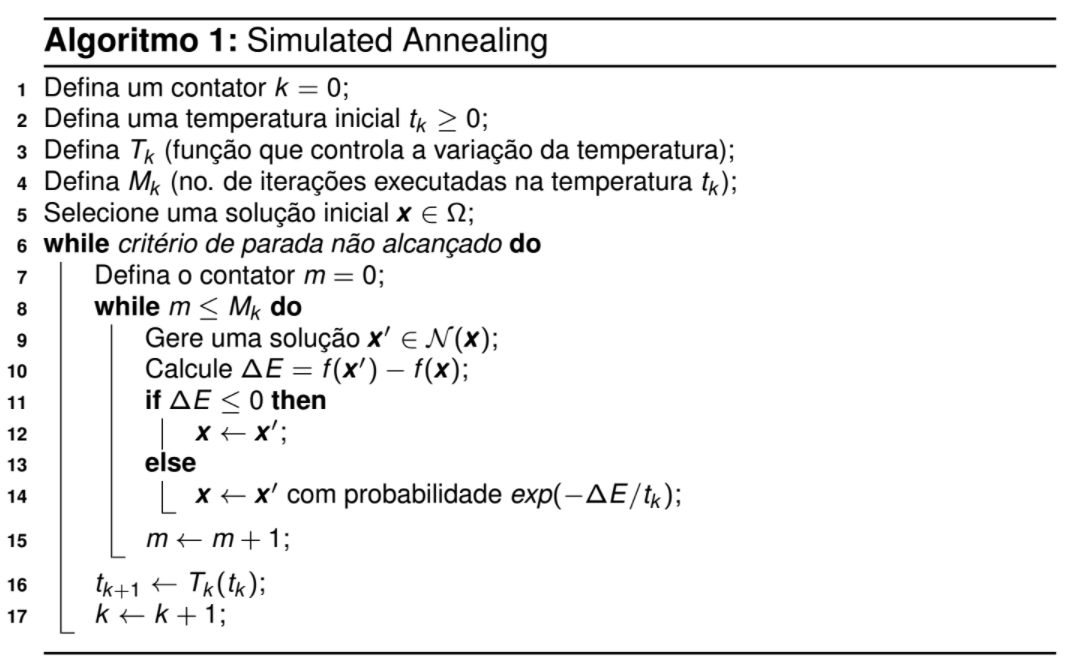
\includegraphics[width=15cm]{img/a.png}
		\caption{Algoritmo simplificado do SA.}
		\label{fig:algoritmo}
	\end{figure}
	
Para tratar o problema da minimização do tempo de entrega, é importante ter em mente a representação de uma possível solução. Esta representação, como discutido na seção A.1, é uma matriz de zeros e uns, onde o 1 representa qual máquina faz dada tarefa.

A primeira etapa foi criar um algoritmo que gera uma solução inicial. Este código está no arquivo \textit{initialSolTE.m}. Uma solução é inicializada como sendo uma matriz de zeros. Então, para cada linha (tarefa), um número randômico entre 1 e a quantidade de máquinas é gerado, representado qual é a máquina escolhida para executar a tarefa daquela linha. Um número 1 é colocado na posição da linha do número randômico gerado. Repare que esta solução gerada nunca viola a restrição de que a soma dos valores de uma linha deve ser sempre 1.

Em seguida, criou-se um código que é responsável por avaliar uma dada solução na função objetivo, algoritmo este que está no arquivo \textit{fobjTE.m}. Este arquivo define a função fobjTE que recebe como entrada a solução que se deseja avaliar e uma matriz com o tempo que cada máquina demora para executar cada tarefa (estes tempos são carregados do arquivo \textit{i5x25.mat} disponibilizado pelo professor). Pela multiplicação vetorial de cada linha da matriz dos tempos com cada coluna da matriz $x$ (solução), tem-se o tempo de operação de cada máquina. A avaliação da solução na função objetivo é, como já visto, o maior dentre os tempos de operação das máquinas.

Antes de implementar o SA propriamente dito, foi necessário também criar funções que geram novas soluções em dada vizinhança. Para este trabalho, duas funções de vizinhança foram criadas. A primeira, para uma dada solução $x$, gera uma nova solução $y$ trocando aleatoriamente as máquinas que executam $n$ tarefas ($n$ também é um parâmetro da função), e está no arquivo \textit{neighbor1TE.m}. Repare que aqui não ocorre necessariamente uma troca entre máquinas. A outra função de vizinhança recebe uma solução $x$ e gera uma nova solução $y$ escolhendo duas linhas aleatoriamente (duas tarefas), e trocando-as, de forma que duas máquinas trocam as tarefas entre si. Está no arquivo \textit{neighbor2TE.m}.
% Reminder: the "draftcls" or "draftclsnofoot", not "draft", class option
% should be used if it is desired that the figures are to be displayed while
% in draft mode.

% An example of a floating figure using the graphicx package.
% Note that \label must occur AFTER (or within) \caption.
% For figures, \caption should occur after the \includegraphics.
%
%\begin{figure}
%\centering
%\includegraphics[width=2.5in]{myfigure}
% where an .eps filename suffix will be assumed under latex, 
% and a .pdf suffix will be assumed for pdflatex
%\caption{Simulation Results}
%\label{fig_sim}
%\end{figure}


% An example of a double column floating figure using two subfigures.
%(The subfigure.sty package must be loaded for this to work.)
% The subfigure \label commands are set within each subfigure command, the
% \label for the overall fgure must come after \caption.
% \hfil must be used as a separator to get equal spacing
%
%\begin{figure*}
%\centerline{\subfigure[Case I]{\includegraphics[width=2.5in]{subfigcase1}
% where an .eps filename suffix will be assumed under latex, 
% and a .pdf suffix will be assumed for pdflatex
%\label{fig_first_case}}
%\hfil
%\subfigure[Case II]{\includegraphics[width=2.5in]{subfigcase2}
% where an .eps filename suffix will be assumed under latex, 
% and a .pdf suffix will be assumed for pdflatex
%\label{fig_second_case}}}
%\caption{Simulation results}
%\label{fig_sim}
%\end{figure*}



% An example of a floating table. Note that, for IEEE style tables, the 
% \caption command should come BEFORE the table. Table text will default to
% \footnotesize as IEEE normally uses this smaller font for tables.
% The \label must come after \caption as always.
%
%\begin{table}
%% increase table row spacing, adjust to taste
%\renewcommand{\arraystretch}{1.3}
%\caption{An Example of a Table}
%\label{table_example}
%\begin{center}
%% Some packages, such as MDW tools, offer better commands for making tables
%% than the plain LaTeX2e tabular which is used here.
%\begin{tabular}{|c||c|}
%\hline
%One & Two\\
%\hline
%Three & Four\\
%\hline
%\end{tabular}
%\end{center}
%\end{table}


\section{Conclusion}
The conclusion goes here.

% conference papers do not normally have an appendix

% use section* for acknowledgement
\section*{Acknowledgment}
% optional entry into table of contents (if used)
%\addcontentsline{toc}{section}{Acknowledgment}
The authors would like to thank...

% trigger a \newpage just before the given reference
% number - used to balance the columns on the last page
% adjust value as needed - may need to be readjusted if
% the document is modified later
%\IEEEtriggeratref{8}
% The "triggered" command can be changed if desired:
%\IEEEtriggercmd{\enlargethispage{-5in}}

% references section
% NOTE: BibTeX documentation can be easily obtained at:
% http://www.ctan.org/tex-archive/biblio/bibtex/contrib/doc/

% can use a bibliography generated by BibTeX as a .bbl file
% standard IEEE bibliography style from:
% http://www.ctan.org/tex-archive/macros/latex/contrib/supported/IEEEtran/bibtex
%\bibliographystyle{IEEEtran.bst}
% argument is your BibTeX string definitions and bibliography database(s)
%\bibliography{IEEEabrv,../bib/paper}
%
% <OR> manually copy in the resultant .bbl file
% set second argument of \begin to the number of references
% (used to reserve space for the reference number labels box)
\begin{thebibliography}{1}

\bibitem{IEEEhowto:kopka}
H.~Kopka and P.~W. Daly, \emph{A Guide to {\LaTeX}}, 3rd~ed.\hskip 1em plus
  0.5em minus 0.4em\relax Harlow, England: Addison-Wesley, 1999.

\end{thebibliography}


% that's all folks
\end{document}


